% === ENCODINGS === 

\usepackage[english, russian]{babel}
\usepackage[T2A]{fontenc}
\usepackage[utf8]{inputenc}

% === MATH === 

% Some math fonts
\usepackage{amsfonts}

% Some math symbols
\usepackage{amssymb}

% Some math "making beautiful" stuff
\usepackage{mathtools}

% Some math fonts
\usepackage{mathrsfs}  

\numberwithin{equation}{section}

% === REFERENCES ===

\usepackage[sorting=none]{biblatex}
\addbibresource{sources.bib}


% === MY COMMANDS ===

\newcommand{\deriv}[2]{\frac{\partial #1}{\partial #2}}
\newcommand{\R}{\mathbb R}
\newcommand{\Row}{\sum\limits_{n=1}^\infty}
\newcommand{\Rowk}{\sum\limits_{k=1}^\infty}
\newcommand{\Prod}{\prod\limits_{n=1}^\infty}
\newcommand{\Prodk}{\prod\limits_{k=1}^\infty}
\newcommand{\eps}{\varepsilon}
\renewcommand{\phi}{\varphi}
\newcommand{\fall}{\:\forall\:}
\newcommand{\ex}{\:\exists\:}

% === MATH OPERATORS ===

\DeclareMathOperator{\const}{const}
\DeclareMathOperator{\Ker}{ker}
\DeclareMathOperator{\Image}{im}
\DeclareMathOperator{\Def}{def}
\DeclareMathOperator{\Rank}{rank}
\DeclareMathOperator{\Dim}{dim}
\DeclareMathOperator{\Argmin}{Argmin}
\DeclareMathOperator{\Tr}{tr}
\DeclareMathOperator{\Interior}{int}
\DeclareMathOperator{\Dom}{dom}
\DeclareMathOperator{\Aff}{aff}
\DeclareMathOperator{\Relint}{relint}

% === OTHER ===

% Indent in the begging of first par
\usepackage{indentfirst}



%==============================================================
\begin{document}

%\title{Использование идей фонтанного кодирования при передаче малого числа битовых пакетов}
\title{ИСПОЛЬЗОВАНИЕ ИДЕЙ ФОНТАННОГО КОДИРОВАНИЯ ПРИ ПЕРЕДАЧЕ МАЛОГО ЧИСЛА БИТОВЫХ ПАКЕТОВ}
\author{\emph{Гуров~С.~И.}\\Московский государственный университет имени М.В. Ломоносова\\
    Факультет Вычислительной математики и кибернетики\\
    Ленинские горы, д.1, стр. 52, Москва, ГСП-1, 119991, Российская Федерация\\
    E-mail: \texttt{sgur@cs.msu.ru}
\and 
\emph{Иванов~Е.~Р.}\\Московский государственный университет имени М.В. Ломоносова\\
    Факультет Вычислительной математики и кибернетики\\
    Ленинские горы, д.1, стр. 52, Москва, ГСП-1, 119991, Российская Федерация\\
    E-mail: \texttt{ivanover@my.msu.ru}}
\date{}

%
\maketitle

%------------------------------------------------------------------------------------------------------------
\textbf{Аннотация.} 
Изучается возможность применения идей фонтанного кодирования для восстановления потерянных пакетов данных при некоторых специальных случаях организации коммуникационной сети.
Предполагается группировка достаточно малого числа битовых пакетов данных в пачки с условием начальной их передачи
<<как есть>> (систематическое кодирование).
Предложены методы решения данной задачи с использованием стохастического подхода и сделаны выводы о их применимости.

\textit{Ключевые слова: систематическое кодирование, потери пакетов в сети, фонтанные коды.}

%----------------------------------------------------------------------------------------------
\section{Введение}
В~конце прошлого века появились технологии, способные передавать чрезвычайно большие объёмы информации
по цифровым сетям передачи данных (телевидение, интернет и др.).
Практически при передаче по телекоммуникационной сети формируются пакеты данных, имеющие одинаковый размер, не превосходящий обычно 
$2^{13}\ldots2^{14}$ бит.

Однако при передаче возможны возникающие на транспортном уровне (по различным причинам) потери отдельных пакетов.
Такими причинами могут быть перегрузки в узлах (коммутаторов, маршрутизаторов и т.~п.), коллизии (наложение пакетов от разных абонентов),
искажения в пакете и др. \cite{Kubickij-2011}.

Для~борьбы с этим явлением обычно применяют автоматический запрос на повторение (\emph{ARQ, Automatic Repeat reQuest}),
при котором принимающее устройство фиксирует наличие ошибок и отправляет запрос устройству-источнику на повторную отправку данных.
Подход носит название \emph{Backward Error Correction} (BEC), и в связи с требуемым в последнее время резким увеличением объёмов и скорости передачи
данных становится все менее приемлемым.

Очевидной альтернативой BEC является применение техники \emph{Forward Error Correction} (FEC).
При этом предполагается группировка пакетов в т.~н. <<пачки>>, и тогда потеря пакета представляется как ошибка его стирания в пачке.
Количество пакетов в пачке может изменятся в широких пределах.
Важно, что место потерянного пакета в составляющей пачку последовательности известно, и возможно применение хорошо известных
методов алгебраического кодирования для исправления ошибок стирания.

Если достаточно обеспечить восстановление небольшого (несколько единиц) числа потерянных пакетов, могут применяться простейшие коды, основанные на добавлении в пачку к \emph{информационным} небольшого числа \emph{проверочных} пакетов, вычисляемых как сумма по $\mod\,2$ от некоторых
информационных.

В~общем случае, казалось бы, можно использовать хорошо изученные принципиально недвоичные коды Рида\,--\,Соломона,
ориентированные на коррекции именно пакетов ошибок \cite{MWill&Sl-79}.
Однако в таких кодах длина кодового слова экспоненциально растёт с увеличением битовой длины символа,
и поэтому практически последний не превосходит 16-и бит (2-х байт).
Поэтому пакет представляется последовательностью из сотен символов, а потеря пакета эквивалентна стиранию всей данной последовательности.
Это приводит к крайне высоким требованиям к исправляющей способности кода и, как следствие, к низкой его скорости
(число информационных символов на один передаваемый).
Поэтому коды Рида\,--\,Соломона, способные исправлять пачки ошибок в отдельно взятом пакете,
<<в случае потери пакета целиком \dots бессильны>> \cite{Shin-Kor-2008}.

Для того, чтобы обойти данное ограничение, приходится использовать пакеты крайне небольшой длины,
дробя исходную полезную нагрузку на большое число частей, что приводит к резкому ухудшению параметров сети передачи данных.

Принципиальным решением рассматриваемой проблемы стало появление т.~н. \emph{фонтанных кодов} (Digital Fountain Codes)
или, по фамилии исследователя, их предложившего, коды Лаби (LT-коды),
применение которых и составляет второй подход её решения \cite{Luby, Mitzenmacher-2004, Kythe2012}.
Эти коды осуществляют преобразование некоторого сообщения конечного размера в потенциально неограниченный поток независимых символов.
Как и в случае простейших кодов стирания, весь пакет рассматривается как единый символ.

Данное свойство рассматриваемых кодов принципиально отличает их от классических помехоустойчивых кодов с заданной скоростью,
когда при кодировании сообщения получается сообщение также конечного размера, а не поток.
Поэтому для кодов из нового класса появился термин \emph{rateless} (нефиксированной скорости) в противовес классическим кодам,
для которых используется термин \emph{fixed rate}.

В~ряде приложений реального времени (потоковое телевещание, системы голосовой связи, онлайн-игр и др.) важно получение приёмником незакодированных пакетов, передаваемых <<как есть>>.
Для решения этой задачи были разработаны \emph{систематические стирающие коды (ССК)} \cite{Shin-Kor-2008}.

Понятие <<систематичности>> для стирающих кодов совпадает с аналогичным в теории блоковых кодов: так называется код, в котором проверочные данные передаются отдельно от исходных данных и исходные данные при кодировании систематическим кодом не изменяются.

%В~статье предложены два алгоритма FEC восстановления потерянных пакетов: фиксированной скорости, гарантирующий восстановление 2 пакетов и фонтанный систематического кодирования.

%----------------------------------------------------------------------------------------------\section{Формулировка проблемы}
\section{Модель канала. Постановка задачи}
В~рассматриваемой модели передатчик формирует пачку из $n$ последовательных пакетов фиксированного размера.
Пакет, кроме данных пользователя (\emph{полезной нагрузки}), содержит и управляющую информацию, необходимую для доставки данных пользователя. 
Для нас важно, что в управляющей информации содержится номер данного пакета в передаваемой пачке.

Приёмник получает, вообще говоря, не все пакеты из пачки, однако номера потерянных пакетов известны.
%
Модель канала передачи данных~--- BEC (Binary Erasure Channel) \cite{Kythe2012}, применённая к пакетам, как символам.
Это означает постоянство 
вероятности $p$ неполучения пакета, что приводит к биномиальному закону
%\begin{equation}\label{eq:Bin(l)}   P(\ell)\,=\,C_n^\ell p^\ell(1-p)^{n-\ell} \end{equation}
$$  
\mathsf P\{\text{стерты } \ell \text{ пакетов}\}\,=\,
\binom{n}{\ell}\, p^\ell(1-p)^{n-\ell},\: 0\le\ell\le n
$$
распределения числа $\ell$ потерянных в пачке из $n$ пакетов.

Далее рассматривается относительно надёжный канал ($p$ мало, например, $p\le0.1$) и случай,
когда по технологическим требованиям пачка не может содержать большого числа пакетов.
Поэтому и возможное число потерянных пакетов в пачке не может быть большим.

Генеральная задача состоит в том, чтобы методами систематического FEC понизить вероятность безвозвратной потери пакета в пачке до значения~$\pi,\:\pi<p$.
Важным ограничением таких подходов является сложность алгоритмов декодирования: над пакетами-символами в несколько тысяч бит
при высоких требованиях к скорости передачи данных реально возможны лишь элементарные операции.

Систематичность кода кажется противоречивым ограничением для фонтанных кодов, которые были спроектированы независящими от порядка посылки символов.
Результат, полученный М.~Лаби в~\cite{Luby}, сформулирован в предельной форме, в ходе доказательства встречаются переходы, верные
при достаточно больших значениях параметров, поэтому на практике LT-коды оказываются полезными при размере пачки порядка тысяч, что делает их неприменимыми в поставленной задаче.

%--------------------------------------------------------------
\section{Формализация и обозначения}

\noindent\textbf{Пакеты данных:} 
    \begin{enumerate}
        \item Пакет -- минимальная неделимая единица информации, при передаче либо
        теряется полностью, либо доходит целиком.
        \item Пакетам присвоены номера от 1 до $k$.
    \end{enumerate}
\noindent\textbf{Отправитель:} 
    \begin{enumerate}
        \item Посылает по сети пронумерованную последовательность пакетов
        с уникальными номерами.
        \item Сначала отправляются все пакеты <<как есть>>, то есть
        первым пересылается первый пакет, вторым -- второй и так далее
        вплоть до $k$-го. 
        \item Далее высылаются $m$ пакетов, каждый из которых 
        формируется по следующему алгоритму: 
        \begin{itemize}
            \item Случайным образом выбирается степень нового кодирующего символа, то есть
            количество суммируемых по модулю 2 пакетов. Формально, генерируется реализация $x$ 
            дискретной случайной величины $X$, имеющей следующее известное отправителю
            распределение:
            \[\mathsf{P}\{X=d\}=\rho(d; k, m), \: d = 1, 2, \dots, k\] 
            \item Случайным образом из $k$ пакетов выбирается 
            $x$-элементное подмножество без возвращений. В силу симметрии задачи 
            относительно перенумеровки пакетов, очевидно, что 
            все $x$-элементные подмножества равновероятны.
            \item Пакеты с выбранными номерами суммируются по модулю 2,
            и результат отправляется получателю. 
        \end{itemize}
    \end{enumerate}
\noindent\textbf{Получатель:}
    \begin{enumerate}
        \item Не имеет никакой связи с отправителем. Известными
        считаются $k$, $m$, а также какие пакеты были просуммированы
        для получения каждого из дошедших проверочных. 
        \item После или по ходу получения пакетов выполняет 
        процедуру декодирования $\mathcal D$.
    \end{enumerate}


\section{Предлагаемые подходы}

Имеющимися степенями свободы являются алгоритм декодирования $\mathcal D$
и распределение $\rho$, по которому высылаются избыточные пакеты.
Возможные различные стратегии распределения сложности между ними.

\subsection{Стратегия сложного алгоритма и простого распределения}

Одним из подходов является использование сложного алгоритма декодирования -- LT-процесса \cite{Luby} -- и малопараметрического распределения.

Выбор возможных распределений степеней кодирующих символов осуществлялся исходя из следующего наблюдения.
Ранее предложенные удачные распределения имеют общее свойство: чаще всего генерируются символы одной и той же степени, которые постепенно
расходуются для поддержания размера очереди.
Перечислим выбранные распределения:

\begin{itemize}

    \item Биномиальное с параметрами $k$ и $\tau$:
        \[
            \rho(d) = \binom{k}{d}\,\tau^d(1-\tau)^{k-d}
        \]
    \item Пуассоновское с параметром $\lambda$:
        \[
            \rho(d) = \frac{\exp\{-\lambda\}\lambda^d}{d!}
        \]
    \item Степень $d^*$ с вероятностью 1:
        \[
            \rho(d) = \delta_{dd^*} = 
            \left\{
            \begin{aligned}
                &1,\: d=d^*\\
                &0,\: d\ne d^*
            \end{aligned}
            \right.
        \]

\end{itemize}

Сделаем несколько замечаний об использовании упомянутых распределений.
В~области значений случайной величины с биномиальным распределением есть ноль, что соответствует кодирующему символу нулевой степени;
с этим недостатком можно, например, бороться с помощью исключения этого значения и последующей перенормировки, однако в данной работе это
не применялось.
Область значений случайной величины с пуассоновским распределением составляет весь натуральный ряд и ноль; для борьбы с возможным символом степени ноль к реализации случайной величины прибавлялась единица, а в случае равенства значению большего $k$ она приравнивалась $k$.

\subsection{Стратегия простого алгоритма и сложного распределения}

\subsubsection{Алгоритм декодирования $\mathcal D$}

Опишем простой алгоритм декодирования. Информационные пакеты декодер
<<просто получает>>, а при обработке проверочных декодирование проводится, 
если множество исходных
пакетов, вошедших в сумму по модулю 2 для формирования полученного
имеет следующую структуру: все, кроме одного -- пришедшие ранее
информационные пакеты.
Данный алгоритм совершает декодирование <<на ходу>> и без памяти, 
то есть каждый
пакет обрабатывается сразу после получения и более декодер никогда
к нему не возвращается.

\subsubsection{Пример}

Пусть имеются пакеты $P_i$, $i=1,\dots, 5$. Отправитель пересылает
через канал их по очереди и до получателя доходят пакеты с номерами
$1, 2, 4$. Далее отправитель пересылает 2 проверочных пакета:
\[C_1 = P_1 \oplus P_2 \oplus P_3\]
\[C_2 = P_1 \oplus P_3 \oplus P_5\]
При получении $C_1$ декодирование будет проведено~--~
получатель восстановит $P_3$, так как все пакеты, кроме $P_3$
-- полученные информационные. При получении $C_2$ декодирование
проведено \emph{не будет}: среди просуммированных пакетов есть 
два не из списка полученных информационных -- $P_3$ и $P_5$. 

Данный пример иллюстрирует возможную нерациональность простого алгоритма:
очевидно, что к моменту получения $C_2$ пакет $P_3$ уже восстановлен
и $P_5$ на самом деле восстановить можно.

\subsubsection{Теория}

Итак, найдем аналитически вероятность того, что произвольный пакет
не будет восстановлен после завершения работы декодера.

Заметим, что модель симметрична относительно перенумеровки пакетов, поэтому
не умаляя общности можно считать, что нас интересует вероятность
безвозвратной утери пакета с номером $k$, а дошедшими при этом можно считать информационные
пакеты с номерами 1, 2, ..., $I$. 

Для каждого вновь прибывшего проверочного пакета вероятность того, что
он восстановит $k$-ый пакет равна
\[\sum_{d=1}^{I + 1}\rho(d)\frac{\binom{I}{d-1}}{\binom{k}{d}}.\]
Формула выше -- формула полной вероятности, первый множитель
каждого слагаемого -- вероятность того, что степень данного 
проверочного пакета равна $d$, второй -- вероятность того, что
все пакеты, кроме одного -- пришедшие информационные при условии, что
степень кодирующего символа равна $d$.

Теперь выпишем выражение для вероятности того, что ни один из $C$ дошедших
проверочных пакетов не восстановил пакет с номером $k$:
\[\left[
    1 - \sum_{d=1}^{I + 1}\rho(d)\frac{\binom{I}{d-1}}{\binom{k}{d}}
\right]^C.\]

Учитывая, что $I$ -- любое число от 0 до $k - 1$,
$C$ -- любое число от 0 до $m$, мы можем выписать итоговую формулу:
\[
\mathsf P\{\text{пакет с номером $k$ не будет восстановлен}\} =
\]
\begin{multline*}
=p\sum_{I=0}^{k-1}\binom{k - 1}{I}\sum_{C=0}^{m}\binom{m}{C}\,
p^{k - 1 + m - I - C}(1-p)^{I + C}\\
\left[
    1 - \sum_{d=1}^{I + 1}\rho(d)\frac{\binom{I}{d-1}}{\binom{k}{d}}
\right]^C =: p\cdot \mathcal L(\rho; k, m) 
\end{multline*}
Множитель $p$ возникает из-за того, что раз пакет с номером
$k$ не восстановлен, значит и как информационный он не был получен. Кроме того,
несложно видеть, что $\mathcal L$ есть вероятность невосстановления пакета
при условии его неполучения.

Для улучшения пропускной способности канала нужно минимизировать функционал $\mathcal L$ по $\bar\rho$, который 
теперь можно считать $k$-мерным вектором из выпуклой оболочки естественного базиса
-- вероятностного симплекса:
\[\bar\rho=(\rho_1, \dots, \rho_k)^\top\equiv
\left[\,\rho(1), \dots, \rho(k)\,\right]^\top\]
\[\rho_i \ge 0, i = 1, \dots, k\]
\[\sum_i \rho_i = 1\]
Число проверочных пакетов $m$ определяет полиномиальную сложность 
поставленной задачи
оптимизации. 

Рассмотрим один частный случай, соответствующий посылке в точности одного 
проверочного пакета ($m=1$).
Стандартным подходом в таком случае является отправка
пакета четности, т.е. суммы по модулю 2 всех пакетов в пачке. Итак,

\[\mathcal L(\bar\rho; k, 1) = \sum_{I=0}^{k-1}\binom{k-1}{I}
p^{k-I}(1-p)^I +\]
\[+ \sum_{I=0}^{k-1}\binom{k-1}{I}
p^{k-I-1}(1-p)^{I+1}
\left[
    1 - \sum_{d=1}^{I + 1}\rho_d\frac{\binom{I}{d-1}}{\binom{k}{d}}
\right]
\]
Нетрудно убедиться в том, что минимизация $\mathcal L$ в этом случае эквивалентна
максимизации 
\[\mathcal L'(\bar\rho; k, 1) = \sum_{I=0}^{k-1}\binom{k-1}{I}p^{k-I-1}(1-p)^{I+1}\sum_{d=1}^{I+1}\rho_d\frac{\binom{I}{d-1}}{\binom{k}{d}}\]
Функционал $\mathcal L'$ линейно зависит от $\rho_1,\dots,\rho_k$,
причем оптимизация проводится на полиэдре. Кроме того, очевидна ограниченность
$\mathcal L'$. Все перечисленное позволяет утверждать, что максимум достигается
в одной из вершин полиэдра. Их конечное число, и все они удовлетворяют
вырожденным распределениям вида
$(0,\dots,0,1,0,\dots,0)^\top$. Таким образом, можно утверждать, что оптимальное
распределение $\rho^*$ имеет следующий вид:
\begin{multline*}
d^* := \underset{\hat d = 1,\dots,k}{\mathrm{Argmin}} 
    \bigg[\frac{1}{\binom{k}{\hat d}}\sum_{I=0}^{k-1}\binom{k-1}{I}\binom{I}{\hat d - 1}\\
    p^{k-I-1}(1-p)^{I+1} \bigg]
\end{multline*}
\[\rho^*(d) = 
    \delta_{dd^*}=
\left\{
\begin{aligned}
    1, \: d = d^* \\
    0, \: d \ne d^*
\end{aligned}\right.\]
Иными словами, отправитель в качестве единственного проверочного пакета посылает
сумму по модулю 2 случайно выбранных $d^*$ пакетов.

\section{Эксперименты}

\subsection{Стратегия сложного алгоритма и простого распределения}

Каждый эксперимент однозначно определяется следующими параметрами: $n$ -- число посылаемых кодирующих символов, $k$ -- число пакетов,
$p$ -- процент потерь в канале и метод кодирования.

В качестве оценки $\hat\pi$ для величины $\pi$ -- достигнутой пропускной способности канала --  использовалось выборочное математическое ожидание:

\[
    \hat\pi = \frac{1}{N_{\mathrm{exps}}}\sum_{j=1}^{N_{\mathrm{exps}}}
    \left[ 1-
    \frac{N^j_{\mathrm{recovered}}}{k} \right],
\]
где $N_{\mathrm{exps}}$ -- число проведенных экспериментов,
$N_{\mathrm{recovered}}^j$ -- число восстановленных пакетов в $j$ реализации.

Результаты экспериментов приведены на рисунках \ref{fig:exp1} и в таблицах
\ref{tab:fountaincodes_results_1}, \ref{tab:fountaincodes_results_2}.
По оси абсцисс отложено математическое ожидание степени каждого кодирующего символа, по оси ординат -- вычисленная оценка $\hat\pi$.
Запись b в таблице означает, что лучшим оказалось биномиальное распределение, d -- вырожденное.

\begin{figure*}[ht]
    \centering
    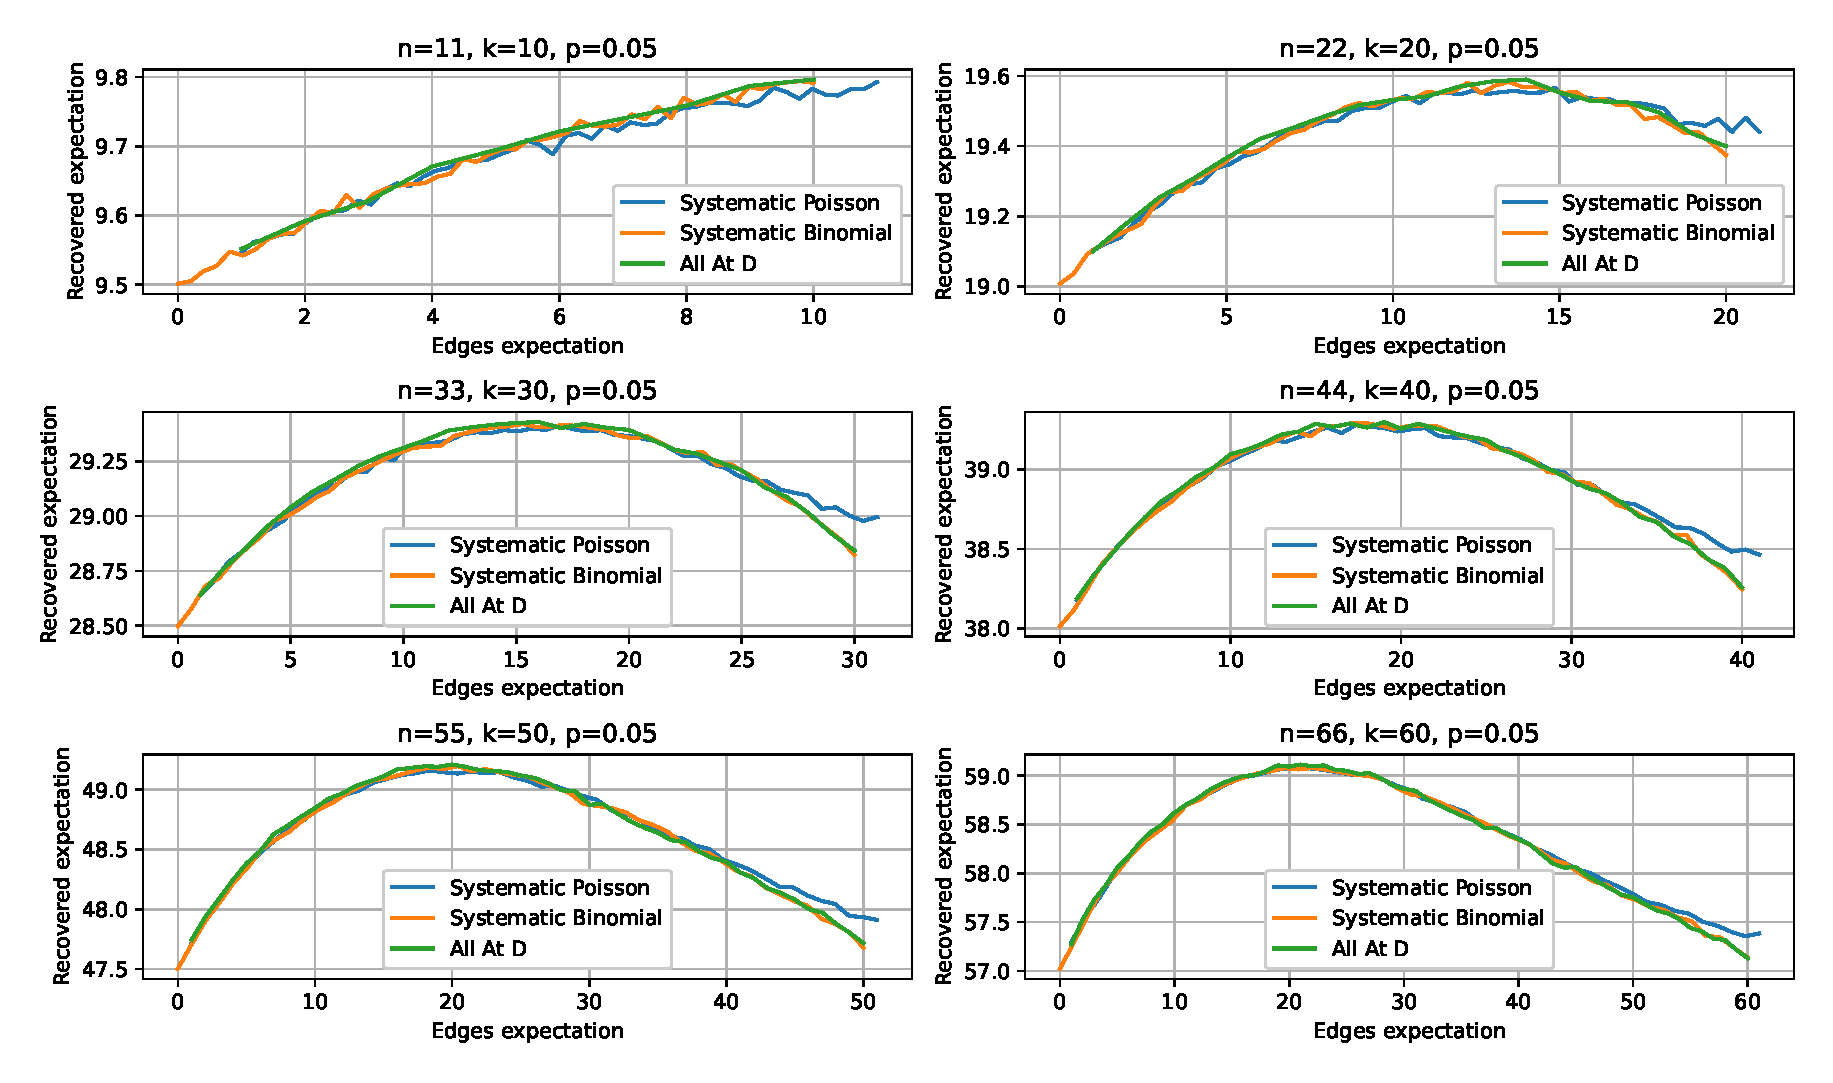
\includegraphics[scale=0.55]{img/exp1.eps}
    \caption{$n=1{,}1k; p=0{,}05$}
    \label{fig:exp1}
\end{figure*}

\begin{table}
\begin{center}
    \begin{tabular}{|c|c|c|c|}
        \hline
        $n$ & $k$ & Метод & $\hat\pi$ \\
        \hline
        12 & 10 & b & 0{,}0123 \\
        \hline
        24 & 20 & d & 0{,}0083 \\
        \hline
        36 & 30 & d & 0{,}0058 \\
        \hline
        48 & 40 & d & 0{,}0041 \\
        \hline
        60 & 50 & d & 0{,}0030 \\
        \hline
        72 & 60 & d & 0{,}0024 \\
        \hline
    \end{tabular}
    \caption{Лучшие результаты методов\\ $p=0{,}05$; избыточность 20\%}
    \label{tab:fountaincodes_results_1}
\end{center}
\end{table}

\begin{table}
\begin{center}
    \begin{tabular}{|c|c|c|c|}
        \hline
        $n$ & $k$ & Метод & $\hat\pi$ \\
        \hline
        12 & 10 & d & 0{,}0221 \\
        \hline
        24 & 20 & d & 0{,}0173 \\
        \hline
        36 & 30 & b & 0{,}0132 \\
        \hline
        48 & 40 & d & 0{,}0100 \\
        \hline
        60 & 50 & d & 0{,}0087 \\
        \hline
        72 & 60 & d & 0{,}0069 \\
        \hline
    \end{tabular}
    \caption{Лучшие результаты методов\\ $p=0{,}07$; избыточность 20\%}
    \label{tab:fountaincodes_results_2}
\end{center}
\end{table}

\subsection{Стратегия простого алгоритма и сложного распределения}

\subsubsection{Случай $m=1$}

Результаты приведены в таблицах \ref{tab:strategy2_results1} и
\ref{tab:strategy2_results2}.

Действительно, при достаточно малых $k$ наиболее вероятна утеря не более, чем одного пакета, 
а значит
можно предположить, что лучшим вариантом будет отправить пакет четности. Однако, с ростом $k$ вероятность того, что 
канал потеряет хотя бы 2 пакета увеличивается и $d^*\ne k$.  

\begin{table}[h!]
\begin{center}
    \begin{tabular}{|c|c|c|c|}
        \hline
        $K$ & $d^*$ & $p \mathcal L$, \% & $\mathcal L^{-1}$ \\
        \hline
        10 & 10 & \textbf{2.01} & \textbf{2.49} \\
        \hline
        15 & 15 & 2.68 & 1.87 \\
        \hline
        20 & 20 & 3.21 & 1.56 \\ 
        \hline
        \textbf{25} & \textbf{19} & 3.57 & 1.40 \\ 
        \hline
        30 & 19 & 3.81 & 1.31 \\
        \hline
    \end{tabular}
    \caption{Результаты экспериментов\\$p=0{,}05, m=1$}
    \label{tab:strategy2_results1}
\end{center}
\end{table}

\begin{table}[h!]
\begin{center}
    \begin{tabular}{|c|c|c|c|}
        \hline
        $K$ & $d^*$ & $p \mathcal L$, \% & $\mathcal L^{-1}$ \\
        \hline
        10 & 10 & \textbf{0.79} & \textbf{3.79} \\
        \hline
        20 & 20 & 1.37 & 2.19 \\
        \hline
        25 & 25 & 1.60 & 1.88 \\ 
        \hline
        30 & 30 & 1.80 & 1.67 \\ 
        \hline
        \textbf{35} & \textbf{33} & 1.96 & 1.53 \\
        \hline
    \end{tabular}
    \caption{Результаты экспериментов\\$p=0{,}03, m=1$}
    \label{tab:strategy2_results2}
\end{center}
\end{table}

\subsubsection{Общий случай: $m>1$}

В общем случае требуется решить задачу условной минимизации функционала на вероятностном симплексе. Результаты  численных экспериментов приведены в таблице \ref{tab:strategy2_results3}, в которых в качестве
метода оптимизации использовался градиентный спуск с проектированием. Проектирование
выполнялось следующим образом: все отрицательные координаты обнулялись, превосходящие
единицу ей приравнивались, после чего выполнялась нормировка. 
Использовались следующие параметры спуска: размер шага: $\alpha=1$, число итераций: 150, 
варианты начального приближения: 

\begin{enumerate}
    \item All-At-Once: 
        \[\bar\rho = (1,0,\dots,0)^\top\] 
    \item Равномерное: 
        \[\rho_i = \frac 1k, \: i = 1,\dots,k\] 
    \item Пакет четности: 
        \[\bar\rho = (0, 0,\dots, 1)^\top\]
\end{enumerate} 

Примеры полученных оптимальных распределений $\bar\rho^*$ приведены на 
рисунках \ref{fig:dist1} и \ref{fig:dist2}.

Под колонкой 
<<Parity Packet Baseline>> подразумевается улучшение пропускной способности
в случае отправки $m$ пакетов четности.

\begin{table}[h!]
\begin{center}
    \begin{tabular}{|c|c|c|c|}
        \hline
        $k$ & $m$ & $p\mathcal L$, \% & Parity Packet Baseline, \% \\
        \hline
        20 & 2 & 1.23 & 1.32 \\
        \hline
        30 & 2 & 1.54 & 1.76 \\
        \hline
        40 & 2 & 1.78 & 2.09 \\
        \hline 
        \hline 
        20 & 3 & 0.93 & 1.32 \\
        \hline
        30 & 3 & 1.23 & 1.76 \\
        \hline
        40 & 3 & 1.47 & 2.09 \\ 
        \hline
        \hline
        20 & 4 & 0.74 & 1.32 \\
        \hline 
        30 & 4 & 1.01 & 1.76 \\
        \hline
        40 & 4 & 1.25 & 2.09\\
        \hline
    \end{tabular}
\caption{Результаты экспериментов\\$p=0{,}03$}
\label{tab:strategy2_results3}
\end{center}
\end{table}

\begin{figure*}[ht]
    \centering
    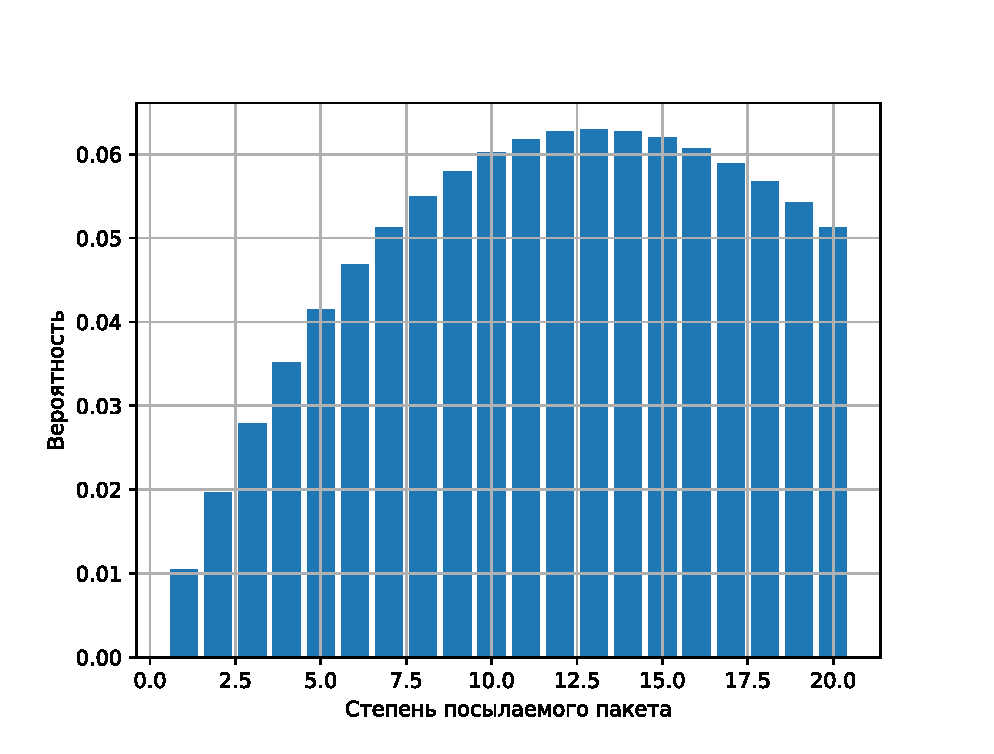
\includegraphics[scale=0.5]{img/distr1.eps}
    \caption{$k=20, \: m=3$}
    \label{fig:dist1}
\end{figure*}

\begin{figure*}[ht]
    \centering
    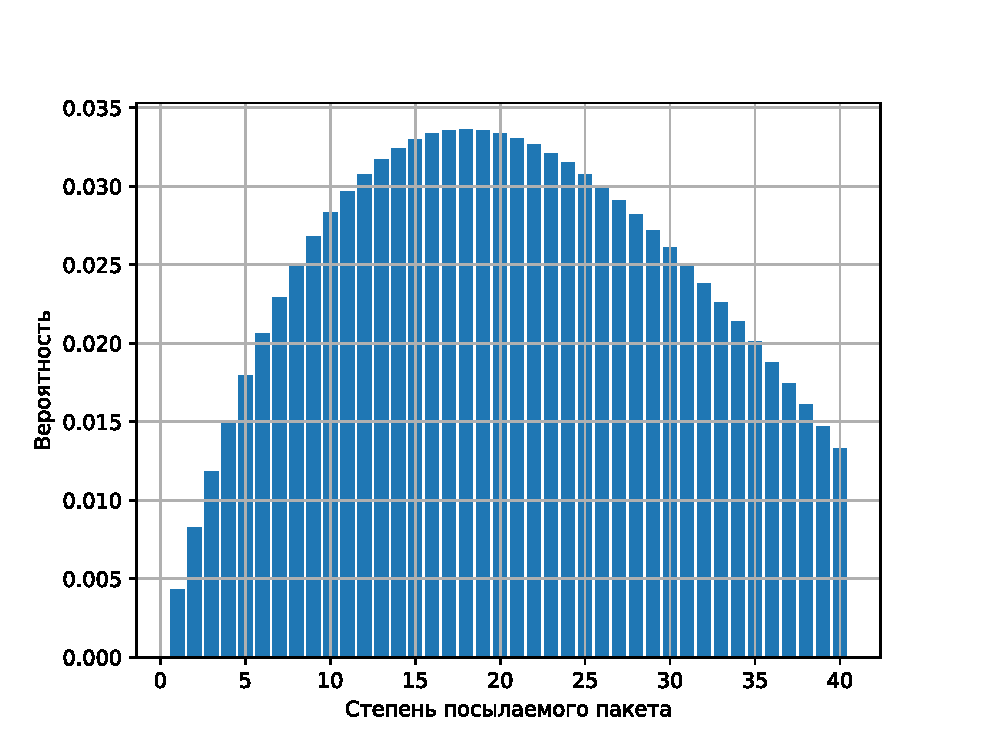
\includegraphics[scale=0.5]{img/distr2.eps}
    \caption{$k=40, \: m=4$}
    \label{fig:dist2}
\end{figure*}

\section{Выводы}

\subsection{Стратегия сложного алгоритма и простого распределения}

Опишем сделанные из экспериментов выводы: для всех распределений верно, что существует единственное значение параметра, при котором оно показывает
наилучший результат;
    наиболее удачным оказался опыт использования вырожденного распределения (кодирующий символ имеет степень $d$ с вероятностью 1);
        оказалось, что вносимая другими распределениями неопределенность в условиях малого количества пакетов скорее мешает, чем помогает;
    до максимума значения растут быстрее, чем падают после; это объяснимо тем, что при малой средней степени генерируемые пакеты
        скорее неинформативны, так как с большой вероятностью полностью <<покрываются>> дошедшими систематическими;
    при больших средних значениях степеней лучше работает пуассоновское распределение; это объяснимо тем, что оно обладает наибольшей дисперсией, а значит при больших средних значениях степеней кодирующие символы меньших степеней будут генеироваться чаще, чем в других
        распределениях.

\subsection{Стратегия простого алгоритма и сложного распределения}

Если методы, соответствующие использованию сложного алгоритма и 
малопараметрического распределения способны снизить вероятность
утери пакета на порядок относительно собственной пропускной способности
канала, то методы, использующие простой алгоритм декодирования 
могут обеспечить улучшение только в 2-3 раза; однако, большим преимуществом таких
методов является очень дешевый процесс декодирования,
совершаемый <<на ходу>> (без памяти), что может быть существенно
для некоторых типов систем передачи информации.

%-----------------------------------------------------------------------------------------------------------------------------------------
\renewcommand{\bibname}{Литература}
\addcontentsline{toc}{section}{\bibname}

\printbibliography[title=Литература]

\end{document}
%======================================================================= 
